\setcounter{subsection}{20-1}
\subsection{The Metric Topology}

\exercise{1}{
  \eparts{
  \item In $\reals^n$, define
    \gath{
      d'(\vx, \vy) = \abs{x_1 - y_1} + \cdots + \abs{x_n - y_n} \,.
    }
    Show that $d'$ is a metric that induces the usual topology of $\reals^n$.
    Sketch the basis elements under $d'$ when $n = 2$.
  \item More generally, given $p \geq 1$, define
    \gath{
      d'(\vx, \vy) = \squares{\sum_{i=1}^n \abs{x_i - y_i}^p}^{1/p}
    }
    for $\vx, \vy \in \reals^n$.
    Assume that $d'$ is a metric.
    Show that it induces the usual topology on $\reals^n$.
  }
}
\sol{
  \dwhitman

  \begin{lem}\label{lem:metric:pmon}
    If $x$ and $y$ are real and $x,y \geq 0$ then $x^p < y^p$ if and only if $x < y$, for all integers $p \geq 1$.
  \end{lem}
  \qproof{
    First, if $x = 0$ then of course
    \gath{
      x < y \bic 0 < y \bic 0 < y^p \bic 0^p < y^p \bic x^p < y^p
    }
    for any $p \geq 1$, so assume it what follows that $x > 0$.
    We show this by induction on $p$.
    First, for $p=1$ we clearly have that $x^p = x$ and $y^p = y$ so that of course the biconditional holds.
    Now suppose that $x^p < y^p$ if and only if $x < y$.
    Suppose that $x < y$ so that $x^p < y^p$ follows by the induction hypothesis.
    We also have that $y > 0$ since $0 < x < y$ so that $y^p > 0$.
    Then
    \ali{
      x^p &< y^p \\
      x \cdot x^p &< x \cdot y^p & \text{(since $x > 0$)} \\
      x \cdot x^p &< x \cdot y^p < y \cdot y^p &  \text{(since $x < y$ and $y^p > 0$)} \\
      x^{p+1} &< y^{p+1} \,.
    }
    Now suppose that it is not true that $x < y$ so that $x \geq y$.
    It then follows from the induction hypothesis that $x^p \geq y^p$.
    Then we have
    \ali{
      x^p &\geq y^p \\
      x \cdot x^p &\geq x \cdot y^p & \text{(since $x > 0$)} \\
      x \cdot x^p &\geq x \cdot y^p \geq y \cdot y^p & \text{(since $x \geq y$ and $y^p \geq 0$ since $y \geq 0$)} \\
      x^{p+1} &\geq y^{p+1} \,.
    }
    Hence by the contrapositive we have that $x^{p+1} < y^{p+1}$ implies that $x < y$.
    This completes the induction.
  }

  \begin{cor}\label{cor:metric:opmon}
    If $x$ and $y$ are real and $x,y \geq 0$ then $x^{1/p} < y^{1/p}$ if and only if $x < y$, for all integers $p \geq 1$.
  \end{cor}
  \qproof{
    Consider any $p \geq 1$ and let $u = x^{1/p}$ and $v = y^{1/p}$.
    Then clearly we have $u,v \geq 0$ since $x,y \geq 0$.
    We then have by Lemma~\ref{lem:metric:pmon} that
    \gath{
      u^p < v^p \bic u < v \\
      (x^{1/p})^p < (y^{1/p})^p \bic x^{1/p} < y^{1/p} \\
      x < y \bic x^{1/p} < y^{1/p} \,,
    }
    which is of course the desired result.
  }

  \begin{lem}\label{lem:metric:polynom}
    For any $n,p \in \pints$ and a finite sequence $\parens{x_i}_{i=1}^n$ where each $x_i \geq 0$,
    \gath{
      \sum_{i=1}^n x_i^p \leq \parens{\sum_{i=1}^n x_i}^p \,.
    }
  \end{lem}
  \qproof{
    For every $n \in \pints$, we show this by induction on $p$.
    For $p = 1$ we clearly have
    \gath{
      \sum_{i=1}^n x_i^p = \sum_{i=1}^n x_i \leq \sum_{i=1}^n x_i = \parens{\sum_{i=1}^n x_i}^p \,.
    }
    Now suppose that the hypothesis is true for $p$.
    Then we have
    \ali{
      \parens{\sum_{i=1}^n x_i}^{p+1} &= \parens{\sum_{i=1}^n x_i}\parens{\sum_{i=1}^n x_i}^p \\
      &\geq \parens{\sum_{i=1}^n x_i}\parens{\sum_{i=1}^n x_i^p} & \text{(by the induction hypothesis since $\sum_{i=1}^n x_i \geq 0$)} \\
      &= \sum_{i=1}^n \sum_{j=1}^n x_i x_j^p \\
      &= \sum_{i=1}^n \parens{x_i x_i^p + \sum_{j \neq i} x_i x_j^p} \\
      &= \sum_{i=1}^n x_i^{p+1} + \sum_{i=1}^n \sum_{j \neq i} x_i x_j^p \\
      &\geq \sum_{i=1}^n x_i^{p+1}
    }
    since each $x_i x_j^p \geq 0$ so that the double sum is as well.
    This completes the induction.
  }

  \mainprob

  (a) First, the basis elements of the metric topology induced by $d'$ are open intervals in $\reals$, open diamonds in $n=2$, open octahedrons for $n = 3$, and the higher dimensional analogues for $n > 3$.
  A sketch of the ball $B_{d'}(0 \times 0, 1)$ in $\reals^2$ is shown below:
  \begin{center}
    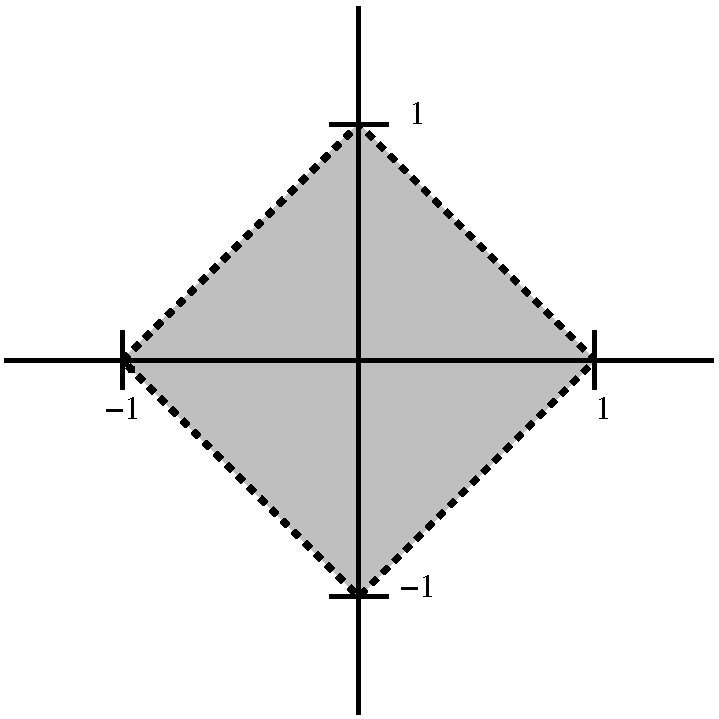
\includegraphics[height=6cm]{figs/ex_20_1_1}
  \end{center}
  Now we show that $d'$ is a metric and induces the usual topology of $\reals^n$.
  \qproof{
    It is easy to see that $d'$ meets the properties required of a metric.
    Clearly $d'(\vx, \vy) \geq 0$ since each $\abs{x_i - y_i} \geq 0$, and $d'(\vx, \vy) = 0$ if and only if each $x_i = y_i$ so that $\vx = \vy$.
    Also it is obvious that $d'(\vx, \vy) = d'(\vy, \vx)$ since each $\abs{x_i - y_i} = \abs{y_i - x_i}$.
    For the triangle inequality we simply have that
    \ali{
      d'(\vx, \vz) &= \sum_{i=1}^n \abs{x_i - z_i} \\
      &\leq \sum_{i=1}^n \parens{\abs{x_i - y_i} + \abs{y_i - z_i}} & \text{(since each $\abs{x_i-z_i} \leq \abs{x_i-y_i} + \abs{y_i-z_i}$)} \\
      &= \sum_{i=1}^n \abs{x_i - y_i} + \sum_{i=1}^n \abs{y_i - z_i} \\
      &= d'(\vx, \vy) + d'(\vy, \vz) \,.
    }

    We now show that the metric topology induced by $d'$ is the same as that induced by the square metric $\r$, which shows the desired result since the square metric induces the standard product topology on $\reals^n$ by Theorem~20.3.
    First consider any $\vx \in \reals^n$ and any $\e > 0$.
    Let $\d = \e$ and consider any $\vy \in B_{d'}(\vx, \d)$.
    Suppose also that $j$ is an index in $\intsfin{n}$ where
    \gath{
      \r(\vx, \vy) = \max\braces{\abs{x_1 - y_1}, \ldots, \abs{x_n - y_n}} = \abs{x_j - y_j} \,.
    }
    Since $\vy \in B_{d'}(\vx, \d)$, we have
    \gath{
      d'(\vx,\vy) = \sum_{i=1}^n \abs{x_i - y_i} < \d = \e \\
      \abs{x_j - y_j} + \sum_{i \neq j} \abs{x_i - y_i} < \e \\
      \abs{x_j - y_j} < \e - \sum_{i \neq j} \abs{x_i - y_i} \leq \e \\
      \r(\vx, \vy) < \e
    }
    since of course $\sum_{i \neq j} \abs{x_i - y_i} \geq 0$.
    Therefore $\vy \in B_\r(\vx,\e)$, which shows $B_{d'}(\vx, \d) \ss B_\r(\vx, \e)$ so that the metric topology of $d'$ is finer the the metric topology of $\r$ by Lemma~20.2.

    Now again consider and $\vx \in \reals^n$ and $\e > 0$, and this time let $\d = \e/n$.
    Consider any $\vy \in B_\r(\vx, \d)$ and again  suppose also that $j$ is an index in $\intsfin{n}$ where
    \gath{
      \r(\vx, \vy) = \max\braces{\abs{x_1 - y_1}, \ldots, \abs{x_n - y_n}} = \abs{x_j - y_j} \,.
    }
    We then have
    \gath{
      \abs{x_j - y_j} = \r(\vx, \vy) < \d = \e/n \\
      n \abs{x_j - y_j} < \e \,.
    }
    We also have
    \ali{
      d'(\vx, \vy) &= \sum_{i=1}^n \abs{x_i - y_i} \\
      &\leq \sum_{i=1}^n \abs{x_j - y_i} & \text{(since each $\abs{x_i - y_i} \leq \abs{x_j - y_j}$)} \\
      &= n \abs{x_j - y_j} \\
      &< \e
    }
    so that $\vy \in B_{d'}(\vx, \e)$.
    Hence $B_\r(\vx, \d) \ss B_{d'}(\vx, \e)$ so that the metric topology of $\r$ is also finer than that of $d'$ again by Lemma~20.2.
    Therefore it must be that the two topologies are equal since each is finer than the other.
  }

  (b) Let $d$ denote the metric defined in part (a), that is
  \gath{
    d(\vx, \vy) = \sum_{i=1}^n \abs{x_i - y_i} \,.
  }
  First we show that the metric topology induced by $d'$ is finer than that induced by $\rho$.
  So consider any $\vx \in \reals^n$ and $\e > 0$.
  Let $\d = \e$ and suppose that $\vy \in B_{d'}(\vx, \d)$ so that
  \gath{
    d'(\vx, \vy) = \parens{\sum_{i=1}^n \abs{x_i - y_i}^p}^{1/p} < \d = \e \,.
  }
  Suppose that $j$ is an index in $\intsfin{n}$ where
  \gath{
    \r(\vx, \vy) = \max\braces{\abs{x_1 - y_1}, \ldots, \abs{x_n - y_n}} = \abs{x_j - y_j} \,.
  }
  Then
  \gath{
    \abs{x_j - y_j}^p \leq \abs{x_j - y_j}^p + \sum_{i \neq j} \abs{x_i - y_i}^p = \sum_{i=1}^n \abs{x_i - y_i}^p
  }
  so that, by Corollary~\ref{cor:metric:opmon}, we have
  \gath{
    \parens{\abs{x_j - y_j}^p}^{1/p} \leq \parens{\sum_{i=1}^n \abs{x_i - y_i}^p}^{1/p} < \e \\
    \abs{x_j - y_j} < \e \\
    \r(\vx, \vy) < \e \,.
  }
  Therefore $\vy \in B_\r(\vx, \e)$ so that $B_{d'}(\vx, \d) \ss B_\r(\vx, \e)$.
  This suffices to show that the metric topology induced by $d'$ is finer than that induced by $\rho$ by Lemma~20.2.

  Now we show that the metric topology induced by $d$ is finer than that induced by $d'$.
  So again consider any $\vx \in \reals^n$ and $\e > 0$.
  Again let $\d = \e$ and suppose that $\vy \in B_d(\vx, \d)$ so that
  \gath{
    d(\vx, \vy) = \sum_{i=1}^n \abs{x_i - y_i} < \d = \e \,.
  }
  Then, since each $\abs{x_i - y_i} \geq 0$, we have by Lemma~\ref{lem:metric:polynom} that
  \ali{
    \sum_{i=1}^n \abs{x_i - y_i}^p &\leq \parens{\sum_{i=1}^n \abs{x_i - y_i}}^p \\
    \parens{\sum_{i=1}^n \abs{x_i - y_i}^p }^{1/p} &\leq \squares{\parens{\sum_{i=1}^n \abs{x_i - y_i}}^p}^{1/p} \\
    d'(\vx, \vy) &\leq \sum_{i=1}^n \abs{x_i - y_i} < \e \,,
  }
  where we have used Corollary~\ref{cor:metric:opmon} in the second step.
  Thus $\vy \in B_{d'}(\vx, \e)$ so that $B_d(\vx, \d) \ss B_{d'}(\vx, \e)$.
  This of course shows that the metric topology induced by $d$ is finer than that induced by $d'$ by Lemma~20.2 again.

  Thus we have shown that the metric topology induced by $d'$ is finer than that induced by $\r$, and also that that induced by $d$ is finer than that induced by $d'$.
  But it was shown in part (a) and Theorem~20.3 that those induced by $d$ and $\r$ are the same topology, which is is the usual product topology on $\reals^n$.
  Hence if $\cT_p$ denotes this usual product topology, we have
  \gath{
    \cT_p = \cT_\r \ss \cT_{d'} \ss \cT_d = \cT_\r = \cT_p \,.
  }
  So it must be that the metric topology induced by $d'$ is this topology as well as desired.
}


\exercise{2}{
  Show that $\reals \times \reals$ in the dictionary order topology is metrizable.
}
\sol{
  \dwhitman

  \qproof{
    In what follows let
    \gath{
      \bd(x,y) = \min\braces{\abs{x-y}, 1}
    }
    be the standard bounded metric on $\reals$, noting that this is a metric by Theorem~20.1.
    Now define the function $d : \reals^2 \times \reals^2 \to \reals$ by
    \gath{
      d(\vx, \vy) = \begin{cases}
        1 & x_1 \neq y_1 \\
        \bd(x_2, y_2) & x_1 = y_1 \,.
      \end{cases}
    }
    We claim that this is a metric on $\reals^2$ that induces the dictionary order topology.

    First we show that $d$ is a metric on $\reals^2$.
    Clearly $d(\vx, \vy) \geq 0$ since both $1 \geq 0$ and $\bd(x_2, y_2) \geq 0$ since $\bd$ is a metric.
    Moreover if $\vx = \vy$ then $x_1 = y_1$ and $x_2 = y_2$ so that $d(\vx, \vy) = \bd(x_2,y_2) = 0$.
    Conversely if $d(\vx, \vy) = 0$ then clearly $d(\vx, \vy) \neq 1$ so that it must be that $x_1 = y_1$ and $d(\vx, \vy) = \bd(x_2,y_2) = 0$ so that $x_2 = y_2$ since $\bd$ is a metric.
    From this it follows that $\vx = \vy$ since $x_1 = y_1$ and $x_2 = y_2$, which shows property (1) of a metric.

    It is also obvious that $d(\vx, \vy) = d(\vy, \vx)$ since if $x_1 \neq y_1$ then $d(\vx,\vy) = 1 = d(\vy, \vx)$.
    If $x_1 = x_2$ then $d(\vx, \vy) = \bd(x_2,y_2) = \bd(y_2,x_2) = d(\vy, \vx)$ since $\bd$ is a metric.
    This shows property (2) of a metric.
    Lastly, consider $\vx$, $\vy$, and $\vz$ in $\reals^2$.

    Case: $x_1 \neq z_1$.
    Then $d(\vx, \vz) = 1$ and it must be that either $y_1 \neq x_1$ or $y_1 \neq z_1$ since otherwise we would have that $x_1 = y_1 = z_1$.
    Thus either $d(\vx, \vy) = 1$ or $d(\vy, \vz) = 1$ and hence
    \gath{
      d(\vx, \vy) + d(\vy, \vz) \geq 1 = d(\vx, \vz)
    }
    since both $d(\vx, \vy) \geq 0$ and $d(\vy, \vz) \geq 0$.

    Case: $x_1 = z_1$.
    Then $d(\vx, \vz) = \bd(x_2,z_2)$.
    If $y_1 = x_1$ then $x_1 = y_1 = z_1$ so that
    \gath{
      d(\vx, \vz) = \bd(x_2,z_2) \leq \bd(x_2,y_2) + \bd(y_2,z_2) = d(\vx,\vy) + d(\vy,\vz)
    }
    since $\bd$ is a metric.
    If $y_1 \neq x_1$ then $y_1 \neq x_1 = z_1$, and hence $d(\vx, \vy) = d(\vy, \vz) = 1$ so that
    \gath{
      d(\vx, \vz) = \bd(x_2, z_2) \leq 1 \leq 2 = 1 + 1 = d(\vx, \vy) + d(\vy, \vz)
    }
    since $\bd$ is the bounded metric so that it is always at most 1.

    Thus in all cases we have shown property (3) of a metric.

    In what follows let $\prec$ denote the dictionary order on $\reals^2$.
    To show that $d$ induces the dictionary order topology, first consider any point $\vx \in \reals^2$ and any basis element $B$ of the dictionary order topology that contains $\vx$.
    Then of course $B = (\va, \vb)$, where $\va \prec \vx \prec \vb$ since the dictionary order has no largest or smallest elements in $\reals^2$.
    Now define
    \gath{
      \d_a = \begin{cases}
        1 & x_2 = a_2 \\
        \abs{x_2 - a_2} & x_2 \neq a_2
      \end{cases}
    }
    and
    \gath{
      \d_b = \begin{cases}
        1 & x_2 = b_2 \\
        \abs{x_2 - b_2} & x_2 \neq b_2 \,,
      \end{cases}
    }
    and let $\d = \min\braces{1, \d_a, \d_b}$.
    Clearly the set $B_d(\vx, \d)$ is a basis element of the topology induced by $d$, and we claim that $\vx \in B_d(\vx, \d) \ss B$.

    That $\vx \in B_d(\vx, \d)$ is obvious.
    So now consider any $\vy \in B_d(\vx, \d)$ so that $d(\vx, \vy) < \d \leq 1$.
    Hence it cannot be that $x_1 \neq y_1$ by definition, since $d(\vx, \vy) = 1$ in that case,  and so $x_1 = y_1$.
    If $x_2 = a_2$ then it has to be that $a_1 < x_1$ since otherwise it would not be the case that $\va \prec \vx$.
    Thus we have $a_1 < x_1 = y_1$ so that $\va \prec \vy$.

    On the other hand if $x_2 \neq a_2$ then it must be that $a_1 \leq y_1$ since otherwise we would have $x_1 = y_1 < a_1$ so that $\vx \prec \va$.
    If $a_1 < y_1 = x_1$ then of course $\va \prec \vy$ so assume that $a_1 = y_1 = x_1$.
    The it must be that $a_2 < x_2$ since $\va \prec \vx$, and so $\abs{x_2 - a_2} = x_2 - a_2$.
    Then, since $x_1 = y_1$, we have that $\bd(x_2, y_2) = d(\vx, \vy) < \d \leq 1$ so it must be that $d(\vx, \vy) = \bd(x_2, y_2) = \abs{x_2 - y_2}$.
    Also $\d_a = \abs{x_2 - a_2} = x_2 - a_2$ since $x_2 \neq a_2$.
    Hence we have $\abs{x_2 - y_2} = d(\vx, \vy) < \d \leq \d_a = x_2 - a_2$, from which it readily follows that $a_2 < y_2$ so that again $\va \prec \vy$.

    Therefore in all cases $\va \prec \vy$.
    Analogous arguments show that $\vy \prec \vb$ so that $\vy \in (\va, \vb) = B$, which shows that $B_d(\vx, \d) \ss B$ as desired since $\vy$ was arbitrary.
    This shows that the topology induced by $d$ is finer than the dictionary order topology by Lemma~13.3.

    Now again suppose that $\vx \in \reals^2$, and that $\e' > 0$ and $\vx' \in \reals^2$ such that $B_d(\vx', \e')$ is an arbitrary basis element of the metric topology induced by $d$ that contains $\vx$.
    It was shown after the definition of a metric topology in the text that there is another ball $B_d(\vx, \e)$ centered at $\vx$ such that $B_d(\vx, \e) \ss B_d(\vx', \e')$.
    Let $\d = \min\braces{1, \e}$ and define $\va = x_1 \times (x_2 - \d)$ and $\vb = x_1 \times (x_2 + \d)$.
    Set $B = (\va, \vb)$, which is clearly a basis element of the dictionary order topology.
    So consider any $\vy \in B$ so that $\va \prec \vy \prec \vb$.
    Clearly it must be that $a_1 = y_1 = b_1 = x_1$ since otherwise we would have that $\vy \prec \va$ or $\vb \prec \vy$.
    From this it follows that $a_2 = x_2 - \d < y_2 < x_2 + \d = b_2$ so that $-\d < y_2 - x_2 < \d$ and hence $\abs{x_2 - y_2} < \d$.
    Moreover, since $y_1 = x_1$ and $\d \leq 1$, it follows that $d(\vx, \vy) = \bd(x_2, y_2) = \abs{x_2 - y_2} < \d \leq \e$.
    This shows that $\vy \in B_d(\vx, \e)$, which shows that $B \ss B_d(\vx, \e) \ss B_d(\vx', \e')$ since $\vy$ was arbitrary.
    This proves that the dictionary order topology is finer than the topology induced by $d$ again by Lemma~13.3.

    Since each is finer than the other the topologies must be the same, which shows that the dictionary order topology is metrizable as desired.
  }
}

\exercise{3}{
  Let $X$ be metric space with metric $d$.
  \eparts{
  \item Show that $d : X \times X \to \reals$ is continuous.
  \item Let $X'$ denote a space having the same underlying set as $X$.
    Show that if $d : X' \times X' \to \reals$ is continuous, then the topology of $X'$ is finer than the topology of $X$.
  }
  One can summarize the result of this exercise as follows: If $X$ has a metric $d$, then the topology induced by $d$ is the coarsest topology relative to which the function $d$ is continuous.
}
\sol{
  \dwhitman

  (a) We use Theorem~18.1 part (4) to show that $d$ is continuous.
  So consider any $x_1 \times x_2 \in X \times X$ and any neighborhood $V$ of $z = d(x_1,x_2)$, noting that $V \ss \reals$ since $\reals$ is the range of $d$.
  Since $V$ is open in $\reals$, there is a basis element $B = (a,b)$ containing $z$ where $B \ss V$.
  Hence $a < z < b$.
  Now let $\e = \min\braces{(z-a)/2, (b-z)/2}$, noting that $\e > 0$ since $z > a$ and $b > z$.
  Next define $U_1 = B_d(x_1, \e)$ and $U_2 = B_d(x_2, \e)$ so that they are both basis elements and therefore open sets of the metric space $X$.
  It then follows that $U = U_1 \times U_2$ is a a basis element and therefore an  open set of the product space $X \times X$.
  Clearly we have that $x_1 \in B_d(x_1, \e) = U_1$ and $x_2 \in B_d(x_2, \e) = U_2$ so that $U$ contains $x_1 \times x_2$ and so is a neighborhood of $x_1 \times x_2$.

  We claim that $d(U) \ss B$.
  To see this, consider any $w \in d(U)$ so that there is a $y_1 \times y_2 \in U = U_1 \times U_2$ such that $w = d(y_1, y_2)$.
  Therefore $y_1 \in U_1 = B_d(x_1, \e)$ so that $d(y_1, x_1) < \e$, and similarly $d(y_2, x_2) < \e$ since $y_2 \in U_2 = B_d(x_2, \e)$.
  Then, since $d$ is a metric, we have
  \ali{
    z = d(x_1, x_2) &\leq d(x_1, y_1) + d(y_1, x_2) \\
    &\leq d(x_1, y_1) + d(y_1, y_2) + d(y_2, x_2) \\
    &= d(y_1, x_1) + d(y_1, y_2) + d(y_2, x_2) \\
    &< \e + w + \e \\
    z &< w + 2\e \leq w + 2(z-a)/2 = w + z - a \\
    a &< w \,.
  }
  Similarly, we have
  \ali{
    w = d(y_1, y_2) &\leq d(y_1, x_1) + d(x_1, y_2) \\
    &\leq d(y_1, x_1) + d(x_1, x_2) + d(x_2, y_2) \\
    &= d(y_1, x_1) + d(x_1, x_2) + d(y_2, x_2) \\
    &< \e + z + \e \\
    w &< z + 2\e \leq z + 2(b-z)/2 = z + b - z \\
    w &< b \,.
  }
  We therefore have that $a < w < b$ so that $w \in (a,b) = B$.
  This of course shows that $d(U) \ss B$ since $w$ was arbitrary.
  Moreover, we have that $B \ss V$ so that clearly $d(U) \ss V$, which completes the proof of Theorem~18.1 part (4) so that $d$ is continuous.

  (b) Let $U$ be any open set of $X$ and consider any $x \in U$.
  Then clearly there is a basis element $B_d(y, \e)$, for some $\e > 0$ and $y \in U$, of the metric topology $X$ that contains $x$ and where $B_d(y, \e) \ss U$.
  Now, since $d$ is continuous with respect to $X' \times X'$, it follows from Exercise~18.11 that the function $d_y(z) = d(y,z)$ is a continuous function from $X'$ to $\reals$.
  Since clearly the interval $(-\infty, \e)$ is open in $\reals$, it then follows that the set
  \gath{
    \inv{d_y}((-\infty, \e)) = \braces{z \in X' \where d_y(z) < \e} = \braces{z \in X \where d(y, z) < \e} = B_d(y, \e)
  }
  is also open in $X'$.
  Thus $B_d(y,\e)$ is an open set in $X'$ containing $x$ such that $B_d(y, \e) \ss U$.
  This shows that $U$ is also open in $X'$ by Exercise~13.1 since the point $x \in U$ was arbitrary.
  This suffices to show the desired result.
}

\exercise{4}{
  Consider the product, uniform, and box topologies on $\reals^\w$,
  \eparts{
  \item In which topologies are the following functions from $\reals$ to $\reals^\w$ continuous?
    \ali{
      f(t) &= (t, 2t, 3t, \ldots), \\
      g(t) &= (t, t, t, \ldots), \\
      h(t) &= (t, \tfrac{1}{2}t, \tfrac{1}{3}t, \ldots).
    }
  \item In which topologies do the following sequences converge?
    \ali{
      \vw_1 &= (1,1,1,1,\ldots), & \vx_1 &= (1,1,1,1, \ldots), \\
      \vw_2 &= (0,2,2,2,\ldots), & \vx_2 &= (0,\tfrac{1}{2},\tfrac{1}{2},\tfrac{1}{2}, \ldots), \\
      \vw_3 &= (0,0,3,3,\ldots), & \vx_3 &= (0,0,\tfrac{1}{3},\tfrac{1}{3}, \ldots), \\
      &\ldots & &\ldots \\
      \vy_1 &= (1,0,0,0,\ldots), & \vz_1 &= (1,1,0,0, \ldots), \\
      \vy_2 &= (\tfrac{1}{2},\tfrac{1}{2},0,0,\ldots), & \vz_2 &= (\tfrac{1}{2},\tfrac{1}{2},0,0, \ldots), \\
      \vy_3 &= (\tfrac{1}{3},\tfrac{1}{3},\tfrac{1}{3},0,\ldots), & \vz_3 &= (\tfrac{1}{3},\tfrac{1}{3},0,0, \ldots), \\
      &\ldots & &\ldots
    }
  }
}
\sol{
  \dwhitman

  \begin{lem}\label{lem:metric:ball}
    Suppose that $X$ is a metric space with metric $d$.
    If $U$ is an open set of $X$ containing a point $x$ then there is a ball $B_d(x, \e)$ centered at $x$ that is contained in $U$.
  \end{lem}
  \qproof{
    The main part of this proof was given after the definition of a metric topology in the text, but we repeat it here for completeness.

    By the definition of the metric topology, there is a $\d > 0$ and $y \in X$ such that the basis element $B_d(y,\d)$ contains $x$ and is contained in $U$.
    Let $\e = \d - d(x,y)$ so that $d(x,y) = \d - \e$, noting that $\e > 0$ since $x \in B_d(y, \d)$ so that $d(x,y) < \d$.
    Then, for any $z \in B_d(x, \e)$, we have that $d(z,x) < \e$ and so
    \gath{
      d(z,y) \leq d(z,x) + d(x,y) = d(z,x) + \d - \e < \e + \d - \e = \d
    }
    since $d$ is a metric.
    Hence $z \in B_d(y, \d)$ so that $B_d(x,\e) \ss B_d(y, \d) \ss U$ as desired since $z$ was arbitrary.
  }

  \begin{lem}\label{lem:metric:finer}
    Suppose that $X$ is a topological space and $Y$ and $Y'$ are topological spaces on the same set, and that $Y'$ is finer than $Y$.
    Suppose also that $f: X \to Y$ so that of course it is also a function from $X$ to $Y'$.
    We assert the following:
    \begin{enumerate}[label=(\arabic*)]
    \item If $f$ is continuous with respect to $Y'$ then it is also continuous with respect to $Y$.
    \item If $f$ is \emph{not} continuous with respect to $Y$ then it is also not continuous with respect to $Y'$.
    \item If a sequence in $Y'$ converges to a point $y_0$, then it also converges to $y_0$ in $Y$.
    \item If a sequence in $Y$ does not converge to a point $y_0$, then it also does not converge to $y_0$ in $Y'$.
    \item If a sequence in $Y$ does not converge at all, then it also does not converge at all in $Y'$.
    \item If $Y$ is a Hausdorff space, then so is $Y'$.
    \end{enumerate}
  \end{lem}
  \qproof{
    For assertion (1) suppose that $f$ is continuous with respect to $Y'$ and let $U$ be any open set of $Y$.
    Since $Y'$ is finer than $Y$, it follows that $U$ is also open in $Y'$.
    Then, since $f$ is continuous with respect to $Y'$ we have that $\inv{f}(U)$ is open in $X$, which suffices to show that $f$ is continuous with respect to $Y$ since $U$ was an arbitrary open set. Assertion (2) follows immediately from the contrapositive of (1).

    Regarding (3), suppose that a sequence $(y_1, y_2, y_3, \ldots)$ converges to $y_0$ in $Y'$ and let $U$ be any neighborhood of $y_0$ in $Y$.
    Then $U$ is also open in $Y'$ since it is finer than $Y$, hence $U$ is a neighborhood of $y_0$ in $Y'$.
    Thus there is an $N \in \pints$ such that $x_n \in U$ for all $n \geq N$, since the sequence converges to $y_0$ in $Y'$.
    Since $U$ was an arbitrary neighborhood of $Y$, this shows that the sequence converges to $y_0$ in $Y$.
    Assertion (4) follows immediately from the contrapositive of (3).
    Assertion (5) then immediately follows from (4) since, if a sequence does not converge at all in $Y$ then for any point $y_0 \in Y$, it does not converge to $y_0$.
    Then it also does not converge to $y_0$ in $Y'$ by (4).
    Since $y_0$ was arbitrary, this shows that it does not converge at all in $Y'$.

    For (6), suppose that $Y$ is a Hausdorff space and let $x$ and $y$ be distinct points of $Y'$ so that they are of course also points of $Y$.
    Hence there are neighborhoods $U$ and $V$ of $x$ and $y$, respectively, in $Y$ that are disjoint.
    Since $Y'$ is finer than $Y$, we have that $U$ and $V$ are also open sets of $Y'$ and thus are disjoint neighborhoods of $x$ and $y$ in $Y'$ as well.
    This suffices to show that $Y'$ is Hausdorff as desired.
  }

  \mainprob
  
  (a) Regarding whether or not the functions are continuous in the various topologies, we claim the following:
  \begin{center}
    \begin{tabular}{c|ccc}
      & Product & Uniform & Box \\
      \hline
      $f$ & Yes & No & No \\
      $g$ & Yes & Yes & No \\
      $h$ & Yes & Yes & No
    \end{tabular}
  \end{center}

  \qproof{
    First, the functions $f$, $g$, and $h$ can all be considered as special cases of the more general function
    \gath{
      s(t) = (s_n(t))_{n \in \pints} \,,
    }
    where each $s_n(t) = \a_n t$, and $\a_n = n$ for $f$, $\a_n = 1$ for $g$, and $\a_n = 1/n$ for $h$.

    Clearly each $s_n$ is continuous for the three $\a_n$ by elementary calculus so that $s$ is continuous in the product topology by Theorem~19.6 for all three $\a_n$.
    We can show that $s$ is \emph{not} continuous in the box topology for all three $\a_n$ with a single example.
    Consider the set $B = \prod_{n \in \pints} (-1/n^2, 1/n^2)$, which is clearly a basis element of the box topology and so is open.
    Similar to Example~19.2, if $s$ were continuous then there would be an interval $(-\d, \d)$ about the point $0$ such that $s((-\d, \d)) \ss B$, where of course $\d > 0$.
    This would of course mean that
    \gath{
      s_n((-\d, \d)) = (-\a_n \d, \a_n \d) \ss (-1/n^2, 1/n^2)
    }
    for all $n \in \pints$.
    However, since clearly there is an $n \in \pints$ large enough that
    \gath{
      n^3 \d \geq n^2 \d \geq n \d > 1 \,,
    }
    we have that
    \gath{
      n\d \geq \d \geq \d/n > 1/n^2 \,,
    }
    and hence for all three functions we have that $\a_n \d > 1/n^2$ so that
    \gath{
      s_n((-\d,\d)) = (-\a_n\d, \a_n \d) \nss (-1/n^2, 1/n^2) \,.
    }
    This shows that $s$ cannot be continuous with respect to the box topology for all three $\a_n$.

    Next we show that $f$ is \emph{not} continuous in the uniform topology.
    First, suppose that $\br$ is the metric that induces the uniform topology, i.e.
    \gath{
      \br(\vx, \vy) = \sup\braces{\bd(x_n, y_n) \where n \in \pints} \,.
    }
    Now consider the basis element and open set $B_{\br}(\vze, 1)$ in the uniform topology.
    If $f$ were continuous then there would be a $\d > 0$ such that
    \gath{
      f((-\d, \d)) = \prod_{n \in \pints} (-\d n, \d n) \ss B_{\br}(\vze, 1) \,.
    }
    Clearly there is an $n \in \pints$ large enough such that $n > 1/\d$ so that $\d n > 1$.
    Then consider the point $\vx \in \reals^\w$ defined by
    \gath{
      x_m = \begin{cases}
        0 & m \neq n+1 \\
        \d n & m = n+1 \,.
      \end{cases}
    }
    We then have of course that $-(n+1)\d < 0 < n\d = x_{n+1} < (n+1)\d$ so that $x_{n+1} \in (-(n+1)\d, (n+1)\d)$.
    It then follows that $\vx \in f((-\d, \d)$.
    However, we also have that $\bd(\d n, 0) = \max\braces{\abs{\d n - 0}, 1} = \max\braces{\d n, 1} = 1$ since $\d n > 1$.
    Hence it is not true that $\br(\vx, \vze) < 1$ so that $\vx \notin B_{\br}(\vze, 1)$.
    Thus $f((-\d, \d)) \nss B_{\br}(\vze, 1)$ so that $f$ is not continuous in the uniform topology.

    Next we show that $g$ and $h$ \emph{are} continuous in the uniform topology at the same time, which we show using Theorem~18.1 part (4).
    Consider any real $u$ and any neighborhood $V$ of $\vx = g(u)$ (or $\vx = h(u)$) in the uniform topology.
    Then by Lemma~\ref{lem:metric:ball} there is an $\e > 0$ such that the basis element $B_{\br}(\vx, \e)$ is a subset of $V$.
    Now consider the basis element and open set $U = B_d(u, \e/2)$, where $d$ denotes the usual metric on $\reals$.
    Obviously $U$ contains $u$ but we also claim that $g(U) \ss V$ (or $h(U) \ss V$), thereby completing the proof.

    So consider any $\vy \in g(U)$ (or $\vy \in h(U)$) so that there is some $v \in U$ such that $\vy = g(v)$ (or $\vy = h(v)$)
    In the case of $g$ we have that $\vx = g(u) = (u,u,u,\ldots)$, which is to say that $x_n = u$ for all $n \in \pints$.
    Similarly $y_n = v$ for all $n \in \pints$ since $\vy = g(v)$.
    Now, since $v \in U = B_d(u,\e/2)$, we have that
    \gath{
      \bd(y_n, x_n) \leq d(y_n, x_n) = d(v, u) < \e/2
    }
    for all $n \in \pints$.
    From this it follows that
    \gath{
      \br(\vy, \vx) = \sup\braces{\bd(y_n, x_n) \where n \in \pints} \leq \e/2 < \e \,.
    }
    Likewise in the case of $h$ we have that $x_n = u/n$ and $y_n = v/n$ for all $n \in \pints$ since $\vx = h(u)$ and $\vy = h(v)$.
    We therefore have that
    \gath{
      \bd(y_n, x_n) \leq d(y_n, x_n) = \abs{y_n - x_n} = \abs{v/n - u/n} = \abs{\frac{v-u}{n}} = \frac{1}{n}\abs{v-u} = \frac{1}{n}d(v,u) < \frac{\e/2}{n} \leq \e/2
    }
    for all $n \in \pints$ since every $n \geq 1$.
    Hence again
    \gath{
      \br(\vy, \vx) = \sup\braces{\bd(y_n, x_n) \where n \in \pints} \leq \e/2 < \e \,.
    }
    Therefore for both functions we have $\br(\vy, \vx) < \e$ so that $\vy \in B_{\br}(\vx, \e)$.
    This shows that $g(U) \ss B_{\br}(\vx, \e) \ss V$ (or $h(U) \ss B_{\br}(\vx, \e) \ss V$) as desired since $\vy$ was arbitrary.
  }

  (b) First we note that, since $\reals$ is a Hausdorff space, $\reals^\w$ is as well in both the box and product topologies by Theorem~19.4.
  Therefore the uniform topology on $\reals^\w$ is also Hausdorff by Lemma~\ref{lem:metric:finer} part (6) since it is finer than the product topology.
  It then follows from Theorem~17.10 that if any of the sequences converge in any of the three topologies, then they converge to a unique point.

  Regarding whether the sequences converge in the various topologies then, we claim
    \begin{center}
    \begin{tabular}{c|ccc}
      & Product & Uniform & Box \\
      \hline
      $\vw$ & Yes & No & No \\
      $\vx$ & Yes & Yes & No \\
      $\vy$ & Yes & Yes & No \\
      $\vz$ & Yes & Yes & Yes
    \end{tabular}
  \end{center}
  \qproof{
    Now, regarding the $\vw$ sequence, each element in the sequence is defined as
    \gath{
      \vw_n = (w_{n,1}, w_{n,2}, w_{n,3}, \ldots) \,,
    }
    where
    \gath{
      w_{n,m} = \begin{cases}
        0 & m < n \\
        n & m \geq n
      \end{cases}
    }
    for $n,m \in \pints$.

    First we show that the $\vw$ sequence converges to the point $\vze$ in the product topology.
    So consider any neighborhood $U$ of $\vze$ in the product topology so that there is a basis element $B$ containing $\vze$ where $B \ss U$.
    Then $B = \prod_{m=1}^\infty B_m$ where each $B_m$ is open and $B_m$ is all of $\reals$ for all but finitely many values of $m$.
    Let $J$ then be a finite subset of $\pints$ where each $B_m = \reals$ for $m \notin J$.
    Of course we also have that $0 \in B_m$ for all $m \in \pints$ since $B$ contains $\vze$.

    Then $J$ has a largest element $N$ since it is a finite set of positive integers.
    Now consider any $n \geq N+1$ and any $m \in \pints$.
    If $m \in J$ then we have that $m \leq N < N+1 \leq n$ since $N$ is the largest element of $J$, and hence $w_{n,m} = 0 \in B_m$.
    If $m \notin J$ then of course $B_m = \reals$ so that of course $w_{n,m} \in \reals = B_m$ regardless of whether $w_{n,m} = 0$ or $w_{n,m} = n$.
    Hence either way we have $w_{n,m} \in B_m$, which shows that $\vw_n \in \prod_{m=1}^\infty B_m = B$ since $m$ was arbitrary.
    Thus also $\vw_n \in U$ since $B \ss U$.
    Since $n \geq N+1$ was arbitrary and $U$ was an arbitrary neighborhood of $\vze$, this shows that the sequence converges to $\vze$ as desired.
    
    Next we show that the $\vw$ sequence does not converge in the uniform topology.
    It suffices to show that the sequence does not converge to $\vze$, since if it converged to any other point $\vx$, then by Lemma~\ref{lem:metric:finer} part (3) it would also converge to $\vx$ in the product topology since it is coarser than the uniform topology.
    However, this would violate the fact that the sequence converges to $\vze$ in the product topology (just shown above), and so cannot also converge to $\vx \neq \vze$ since the convergence point is unique as noted above.

    So consider the neighborhood $B_{\br}(\vze, 1)$ of $\vze$ in the uniform topology.
    We claim that no elements of the sequence are in this neighborhood so that it clearly cannot converge to $\vze$.
    So consider any $n \in \pints$ so that we clearly have $w_{n,n} = n \geq 1 > 0$.
    Therefore $d(w_{n,n}, 0) = \abs{w_{n,n} - 0} = \abs{w_{n,n}} = w_{n,n} \geq 1$, from which it follows that it has to be that $\bd(w_{n,n}, 0) = 1$.
    This of course implies that
    \gath{
      \br(\vw_n, \vze) = \sup\braces{\bd(w_{n,m}, 0) \where m \in \pints} \geq 1 \,.
    }
    Hence it is not true that $\br(\vw_n, \vze) < 1$ so that $\vw_n \notin B_{\br}(\vze, 1)$.
    This shows the desired result since $n$ was arbitrary.

    It then follows that the $\vw$ sequence also does not converge at all in the box topology by Lemma~\ref{lem:metric:finer} part (5) since it is finer than the uniform topology.

    Regarding the $\vx$ sequence, the definition is that each
    \gath{
      \vx_n = (x_{n,1}, x_{n,2}, x_{n,3}, \ldots) \,,
    }
    where
    \gath{
      x_{n,m} = \begin{cases}
        0 & m < n \\
        1/n & m \geq n
      \end{cases}
    }
    for $n,m \in \pints$.

    First we show that this sequence converges to $\vze$ in the uniform topology, which is of course is the unique convergence point.
    So consider any neighborhood $U$ of $\vze$ in the uniform topology so that by Lemma~\ref{lem:metric:ball} there is an $\e > 0$ where $B_{\br}(\vze, \e) \ss U$.
    Then there is a positive integer $N$ large enough so that $N > 2/\e$ so that, for any $n \geq N$ we have $1/n \leq 1/N < \e/2$.
    Next consider any such $n \geq N$ and any $m \in \pints$.
    Since $x_{n,m}$ is either $0$ or $1/n$ we have that $\abs{x_{n,m}} = x_{n,m} \leq 1/n$ so that
    \gath{
      \bd(x_{n,m}, 0) \leq d(x_{n,m}, 0) = \abs{x_{n,m} - 0} = \abs{x_{n,m}} = x_{n,m} \leq 1/n < \e/2 \,.
    }
    Thus, since $m$ was arbitrary, it follows that
    \gath{
      \br(\vx_n, \vze) = \sup\braces{\bd(x_{n,m}, 0) \where m \in \pints} \leq \e/2 < \e \,,
    }
    and hence $\vx_n \in B_{\br}(\vze, \e)$.
    Thus also $\vx_n \in U$ since $B_{\br}(\vze, \e) \ss U$.
    Since $n \geq N$ was arbitrary as was the neighborhood $U$, this shows that the sequence converges to $\vze$ as desired.

    Since it is coarser than the uniform topology, it follows that the $\vx$ sequence also converges to $\vze$ in the product topology as well by Lemma~\ref{lem:metric:finer} part (3).

    Next we show that the $\vx$ sequence does not converge in the box topology, for which it suffices to show that it does not converge to $\vze$.
    Again, this is because, if it were to converge to some other point $\vy \neq 0$ in the box topology, then it would also converge to $\vy$ in the uniform topology since it is coarser (Lemma~\ref{lem:metric:finer} part (3)), but this would violate the fact that it converges to the unique point $\vze$ by what was just shown.
    So consider the basis element and open set of the box topology $U = \prod_{n=1}^\infty U_n$ where each $U_n = (-1/n, 1/n)$.
    Clearly $U$ contains $\vze$ so that it is a neighborhood of $\vze$.
    We claim that no element of the sequence is in $U$, which of course suffices to show that it cannot converge to $\vze$.
    So consider any $n \in \pints$ and so that $x_{n,n} = 1/n \geq 1/n$ so that $x_{n,n} \notin (-1/n, 1/n) = U_n$.
    From this it follows that $\vx_n \notin \prod_{n=1}^\infty U_n = U$.
    Since $n$ was arbitrary this shows no element of the sequence is in $U$ so that the sequence cannot converge to $\vze$.

    Regarding the $\vy$ sequence, it is defined as
    \gath{
      \vy_n = (y_{n,1}, y_{n,2}, y_{n,3}, \ldots) \,,
    }
    where
    \gath{
      y_{n,m} = \begin{cases}
        1/n & m \leq n \\
        0 & m > n
      \end{cases}
    }
    for $n,m \in \pints$.
    Since $y_{n,m}$ is always either $0$ or $1/n$, the same argument that shows that the $\vx$ sequence converges to $\vze$ in the uniform topology shows that the $\vy$ sequence does as well.
    Of course this also mean that it converges to $\vze$ in the product topology as well since it is coarser.
    Similarly, the same argument that shows that the $\vx$ sequence does not converge in the box topology applies to $\vy$ as well since we have that $y_{n,n} = x_{n,n} = 1/n$ for all $n \in \pints$.

    Now, the $\vz$ sequence is defined by
    \gath{
      \vz_n = (z_{n,1}, z_{n,2}, z_{n,3}, \ldots) \,,
    }
    where
    \gath{
      z_{n,m} = \begin{cases}
        1/n & m \leq 2 \\
        0 & m > 2
      \end{cases}
    }
    for $n,m \in \pints$.

    We show that this sequence converges to $\vze$ in the box topology.
    So consider any neighborhood $U$ of $\vze$ in the box topology so that there is a basis element $B = \prod_{m=1}^\infty B_m$ containing $\vze$ where $B \ss U$.
    Of course then each $B_m$ is open in $\reals$ and $0 \in B_m$.
    Considering the standard topology of $\reals$ using the metric topology basis, there is then an $\e_1 > 0$ such that $B_d(0, \e_1) \ss B_1$ by Lemma~\ref{lem:metric:ball} since $B_1$ is open and contains $0$.
    Likewise there is an $\e_2 > 0$ where $B_d(0, \e_2) \ss B_2$.
    So set $\e = \min\braces{\e_1, \e_2}$ so that of course there is a positive integer $N$ large enough that $N > 1/\e$.
    Then, for any $n \geq N$ we have that $n \geq N > 1/\e$ so that $1/n < \e \leq \e_1$, and similarly $1/n < \e \leq \e_2$.
    Now consider any $m \in \pints$.
    If $m \leq 2$ then of course either $m = 1$ or $m = 2$ so that, either way, we have
    \gath{
      d(z_{n,m}, 0) = \abs{z_{n,m} - 0} = \abs{z_{n,m}} = \abs{1/n} = 1/n < \e \leq \e_m
    }
    so that $z_{n,m} \in B_d(0, \e_m) \ss B_m$.
    If $m > 2$ then we clear have $z_{n,m} = 0 \in B_m$ as well.
    Since $m$ was arbitrary, this shows that $\vz_n \in \prod_{m=1}^\infty B_m = B \ss U$.
    This shows that the sequence converges to $\vze$ since $n \geq N$ was arbitrary and $U$ was any neighborhood of $\vze$.

    Of course this also shows that the $\vz$ sequence converges to $\vze$ in the uniform and product topologies as well by Lemma~\ref{lem:metric:finer} part (3) since they are both coarser than the box topology.
  }
}

\exercise{5}{
  Let $\rinf$ be the subset of $\reals^\w$ consisting of all sequences that are eventually zero.
  What is the closure of $\rinf$ in $\reals^\w$ in the uniform topology?
  Justify your answer. 
}
\sol{
  \dwhitman

  Let $\reals^0$ denote the subset of $\reals^\w$ consisting of all sequences that converge to zero.
  We then claim that $\closure{\rinf} = \reals^0$, i.e. the closure of $\rinf$ is $\reals^0$.
  \qproof{
    $(\ss)$ We show this by contrapositive.
    So suppose that $\vx \notin \reals^0$ so that the sequence $\vx$ does \emph{not} converge to zero.
    Then there is a neighborhood $V$ of $0$ in the standard topology on $\reals$ such that, for any $N \in \pints$, there is an $n \geq N$ where $x_n \notin V$.
    It also follows from Lemma~\ref{lem:metric:ball} that there is an $\e > 0$ such that $B_d(0, \e) \ss V$.
    So let $\d = \min\braces{\e, 1}$ and consider the set $B_{\br}(\vx, \d)$, which is clearly a neighborhood of $\vx$ in the uniform topology.
    Also suppose that $\vy$ is any element of $\rinf$ so that $\vy$ is eventually zero.
    Then there must be an $N$ where $y_n = 0$ for all $n \geq N$.
    From before we have that there is a specific $n \geq N$ where $x_n \notin V$ so that also $x_n \notin B_d(0, \e)$, and thus
    \gath{
      d(y_n, x_n) = d(0, x_n) = d(x_n, 0) \geq \e \geq \d \,.
    }
    Then we have that both $d(y_n, x_n) \geq \d$ and $1 \geq \d$ so that
    \gath{
      \bd(y_n, x_n) = \min\braces{d(y_n, x_n), 1} \geq \d \,.
    }
    From this it clearly follows that
    \gath{
      \br(\vy, \vx) = \sup\braces{\bd(y_n, x_n) \where n \in \pints} \geq \d
    }
    so that $\vy \notin B_{\br}(\vx, \d)$.
    Since $\vy$ was arbitrary, this shows that $B_{\br}(\vx, \d)$ does not intersect $\rinf$.
    This in turn shows that $\vx$ is not a limit point of $\rinf$.
    Now, clearly also $\vx$ cannot be eventually zero since then it would converge to zero, hence $\vx \notin \rinf$ either.
    Therefore $\vx$ cannot be in the closure of $\rinf$.
    Hence by the contrapositive we have that $\closure{\rinf} \ss \reals^0$.

    $(\sps)$ Now consider any $\vx \in \reals^0$ so that the sequence $\vx$ converges to zero.
    Consider any neighborhood $U$ of $\vx$ in the uniform topology so that, by Lemma~\ref{lem:metric:ball}, there is an $\e > 0$ such that $B_{\br}(\vx, \e) \ss U$.
    Now, since $B_d(0, \e/2)$ is a neighborhood of $0$, it follows that there is an $N \in \pints$ where $x_n \in B_d(0, \e/2)$ for all $n \geq N$ since $\vx$ converges to $0$.
    Now define the sequence $\vy$ where
    \gath{
      y_n = \begin{cases}
        x_n & n < N \\
        0 & n \geq N
      \end{cases}
    }
    for $n \in \pints$.
    Clearly $\vy$ is eventually zero so that $\vy \in \rinf$.

    We also claim that $\vy \in U$.
    To see this consider any $n \in \pints$.
    If $n < N$ then clearly $y_n = x_n$ so that
    \gath{
      \bd(y_n, x_n) \leq d(y_n, x_n) = d(x_n, x_n) = 0 < \e/2 \,.
    }
    If $n \geq N$ then $y_n = 0$ and we have from before that $x_n \in B_d(0, \e/2)$ and hence
    \gath{
      \bd(y_n, x_n) \leq d(y_n, x_n) = d(0, x_n) = d(x_n, 0) < \e/2 \,.
    }
    Hence it follows that
    \gath{
      \br(\vy, \vx) = \sup\braces{\bd(y_n, x_n) \where n \in \pints} \leq \e/2 < \e
    }
    so that $\vy \in B_{\br}(\vx, \e) \ss U$.
    This shows that $\vy \in \rinf \cap U$.
    If $\vy = \vx$ then of course $\vx = \vy \in \rinf$ itself.
    If $\vy \neq \vx$ then we have shown that $\vx$ is a limit point of $\rinf$ since $U$ was an arbitrary neighborhood.
    Thus either way $\vy \in \closure{\rinf}$ so that $\closure{\rinf} \sps \reals^0$ since $\vx$ was arbitrary.
  }
  Lastly, we note that $\rinf$ is a proper subset of its closure $\closure{\rinf} = \reals^0$ since, for example, the sequence $\vx$ defined by $x_n = 1/n$ for all $n \in \pints$ clearly converges to zero so is in $\reals^0$ but is not eventually zero so is not in $\rinf$.
}

\exercise{6}{
  Let $\br$ be the uniform metric on $\reals^\w$.
  Given $\vx = (x_1,x_2,\ldots) \in \reals^\w$ and given $0 < \e < 1$, let
  \gath{
    U(\vx, \e) = (x_1-\e, x_1+\e) \times \cdots \times (x_n - \e, x_n + \e) \times \cdots \,.
  }
  \eparts{
  \item Show that $U(\vx, \e)$ is not equal to the $\e$-ball $B_{\br}(\vx, \e)$.
  \item Show that $U(\vx, \e)$ is not even open in the uniform topology.
  \item Show that
    \gath{
      B_{\br}(\vx, \e) = \bigcup_{\d < \e} U(\vx, \d) \,.
    }
  }
}
\sol{
  \dwhitman

  (a)
  \qproof{
    We show that $B_{\br}(\vx, \e)$ is not a subset of $U(\vx, \e)$, which of course suffices to show that they cannot be equal.
    To this end we define the point $\vy$ in $\reals^\w$ by
    \gath{
      y_n = x_n + \e\parens{1 - \frac{1}{n}}
    }
    for any $n \in \pints$.
    Then, for any such $n$, we clearly have that
    \ali{
      n &\geq 1 \\
      -n &\leq -1 < 0 \\
      -1 &\leq -\frac{1}{n} < 0 & \text{(since $n > 0$)} \\
      0 &\leq 1 - \frac{1}{n} < 1 \\
      0 &\leq \e\parens{1 - \frac{1}{n}} < \e & \text{(since $\e > 0$)} \\
      x_n &\leq x_n + \e\parens{1 - \frac{1}{n}} < x_n + \e \\
      x_n - \e < x_n &\leq y_n < x_n + \e
    }
    so that $y_n \in (x_n - \e, x_n + \e)$.
    Since $n$ was arbitrary, this shows that $\vy \in \prod_{n=1}^\infty (x_n - \e, x_n + \e) = U(\vx, \e)$.
    However, again for any $n \in \pints$, it was shown that $x_n \leq y_n$  so that
    \gath{
      d(y_n, x_n) = \abs{y_n - x_n} = y_n - x_n = x_n + \e\parens{1 - \frac{1}{n}} - x_n = \e\parens{1 - \frac{1}{n}} \,.
    }
    It was shown above that
    \ali{
      0 \leq \e\parens{1 - \frac{1}{n}} < \e &< 1 \\
      0 \leq d(y_n, x_n) < \e &< 1
    }
    so that
    \gath{
      \bd(y_n, x_n) = \min\braces{d(y_n, x_n), 1} = d(y_n, x_n) \,.
    }
    We then clearly have
    \gath{
      \lim_{n \to \infty} \bd(y_n, x_n) = \lim_{n \to \infty} d(y_n, x_n) = \lim_{n \to \infty} \e \parens{1 - \frac{1}{n}} = \e
    }
    so that
    \gath{
      \br(\vy, \vx) = \sup_{n \in \pints} \bd(y_n, x_n) = \e \geq \e
    }
    since the sequence $\vy$ is clearly monotonically increasing.
    This shows that $\vy \notin B_{\br}(\vx, \e)$ so that $B_{\br}(\vx, \e)$ cannot be a subset of $U(\vx, \e)$.
  }

  (b)
  \qproof{
    Let $\vy$ be the point in $\reals^\w$ defined in part (a) so that we know that $\vy \in U(\vx, \e)$.
    Now if $U(\vx, \e)$ were open in the uniform topology then there would be a basis element $B_{\br}(\vy, \d)$ that is contained in $U(\vx, \e)$.
    We shall show that any such basis element cannot be contained within $U(\vx, \e)$, from which the desired result follows.

    So consider any $\d > 0$ so that there is an $n \in \pints$ large enough that $n > \e/\d$.
    Then we have
    \ali{
      n &> \frac{\e}{\d} \\
      \d &> \e \frac{1}{n} & \text{(since both $\d > 0$ and $n > 0$)} \\
      -\e\frac{1}{n} + \d &> 0 \\
      \e - \e\frac{1}{n} + \d &> \e \\
      x_n + \e\parens{1 - \frac{1}{n}} + \d &> x_n + \e \\
      y_n + \d &> x_n + \e \,.
    }
    Now define the point $\vz$ by
    \gath{
      z_m = \begin{cases}
        y_m & m \neq n \\
        \frac{(x_n + \e) + (y_n + \d)}{2} & m = n \,.
      \end{cases}
    }
    It then follows that $x_n + \e < z_n < y_n + \d$.
    The fact that $x_n + \e < z_n$ means that of course $z_n \notin (x_n - \e, x_n + \e)$ so that $\vz \notin \prod_{m=1}^\infty (x_m - \e, x_m + \e) = U(\vx, \e)$.
    However, for $m \neq n$ we have that
    \gath{
      d(z_m, y_m) = d(y_m, y_m) = 0
    }
    and so $\bd(z_m, y_m) = 0$ as well.
    For $m = n$ we have
    \gath{
      x_m + \e = x_n + \e < z_m = z_n < y_n + \d = y_m + \d \\
      x_m + \e - y_m < z_m - y_m < \d \\
      x_m + \e - x_m - \e\parens{1 - \frac{1}{n}} < z_m - y_m < \d \\
      0 < \e\frac{1}{n} < z_m - y_m < \d \\
      \abs{z_m - y_m} < \d \\
      \bd(z_m, y_m) \leq d(z_m, y_m) < \d \,.
    }
    From these facts it follows that
    \gath{
      \br(\vz, \vy) = \sup_{m \in \pints} \bd(z_m, y_m) = \bd(z_n, y_n) < \d
    }
    so that $\vz \in B_{\br}(\vy, \d)$.
    This shows that $B_{\br}(\vy, \d)$ is not a subset of $U(\vx, \e)$, which shows the desired result as explained before.
  }

  (c)
  \qproof{
    $(\ss)$ Let $\vy$ be any element of $B_{\br}(\vx, \e)$ so that $\br(\vy, \vx) < \e$.
    Then there is a $\d$ where $\br(\vy, \vx) < \d < \e$ since the reals are order-dense.
    For any $n \in \pints$ it must be that $\bd(y_n, x_n) < \d < \e < 1$ since $\br$ is the supremum of these.
    From this it has to be that $\bd(y_n, x_n) = d(y_n, x_n) < \d$ so that
    \gath{
      d(y_n, x_n) = \abs{y_n - x_n} < \d \\
      -\d < y_n - x_n < \d \\
      x_n - \d < y_n < x_n + \d \,.
    }
    Hence $y_n \in (x_n - \d, x_n + \d)$.
    Since $n$ was arbitrary, this shows that $\vy \in \prod_{n=1}^\infty (x_n-\d, x_n+\d) = U(\vx, \d)$.
    Thus obviously $\vy \in \bigcup_{\d < \e} U(\vx, \d)$, which shows the desired result.

    $(\sps)$ Now suppose that $\vy \in \bigcup_{\d < \e} U(\vx, \d)$ so that there is a $\d < \e$ where $\vy \in U(\vx, \d)$.
    Consider any $n \in \pints$ so that we have $y_n \in (x_n-\d, x_n+\d)$.
    Then of course
    \gath{
      x_n - \d < y_n < x_n + \d \\
      -\d < y_n - x_n < \d
    }
    so that $d(y_n, x_n) = \abs{y_n - x_n} < \d < \e < 1$ so that it must be that $\bd(y_n, x_n) = d(y_n, x_n) < \d$.
    Since $n$ was arbitrary, it follows that
    \gath{
      \br(\vy, \vx) = \sup\braces{\bd(y_n, x_n) \where n \in \pints} \leq \d < \e \,,
    }
    and hence $\vy \in B_{\br}(\vx, \e)$.
    Since $\vy$ was arbitrary, this shows that $B_{\br}(\vx, \e) \sps \bigcup_{\d < \e} U(\vx, \d)$, which completes the proof.
  }
}

\exercise{7}{
  Consider the map $h: \reals^\w \to \reals^\w$ defined in Exercise~8 of $\S 19$; give $\reals^\w$ the uniform topology.
  Under what conditions on the numbers $a_i$ and $b_i$ is $h$ continuous?
  a homeomorphism?
}
\sol{
  \dwhitman

  First some discussion.
  We know that the product topology is strictly finer than the uniform topology in $\reals^\w$, and the that box topology is strictly finer than the uniform topology.
  By Lemma~\ref{lem:metric:finer} part (1), when the topology on the range of a function becomes coarser, the function remains continuous.
  It is similarly easy to show that if the topology on the \emph{domain} of a function becomes \emph{finer}, it also remains continuous.
  However, nothing can be said for sure if the range becomes finer and/or the domain becomes coarser.

  It was shown in Exercise~19.8 that $h$ is a homeomorphism (for $a_i > 0$ as in the exercise) if both the domain and range have the product topology, or if they both have the box topology.
  By what was just discussed then, $h$ is at least continuous with box topology on the domain, and the uniform topology on the range, or likewise with the uniform topology on the domain and the product topology on the range.
  However, the relative ``fineness'' of these topologies does not allow us to conclude anything about whether $h$ is continuous or a homeomorphism when both the domain and range are the uniform topologies, which is unfortunately what we are interested in.

  In fact, we claim that $h$ is continuous with the uniform topology as the domain and range if and only if the set of numbers $\braces{a_i}_{i \in \pints}$ is bounded (and of course each $a_i > 0$).
  \qproof{
    $(\imp)$ We show this direction by contrapositive.
    So suppose that $\braces{a_i}$ is not bounded.
    We then show that $h$ is not continuous by showing the negation of Theorem~18.1 part (4).
    So consider the point $\vze$ and the neighborhood $V = B_{\br}(h(\vze), 1)$ in the uniform topology.
    Consider also any neighborhood $U$ of $\vze$ so that by Lemma~\ref{lem:metric:ball} there is an $\e > 0$ where $B_{\br}(\vze, \e) \ss U$.
    Now define the point $\vx \in \reals^\w$ by $x_i = \e/2$ for all $i \in \pints$.
    Then, for any $i \in \pints$, we have
    \gath{
      \bd(x_i, 0) \leq d(x_i, 0) = \abs{x_i - 0} = \abs{x_i} = \abs{\e/2} = \e/2
    }
    so that clearly
    \gath{
      \br(\vx, \vze) = \sup\braces{\bd(x_i, 0) \where i \in \pints} \leq \e/2 < \e \,,
    }
    and hence $\vx \in B_{\br}(\vze, \e)$ so that also $\vx \in U$.
    Then clearly $h(\vx) \in h(U)$.

    Now, since the $a_i$ coefficients are unbounded, there is a specific $i \in \pints$, where $a_i \geq 2/\e$ regardless of how small $\e$ is.
    We then have that
    \gath{
      d(h_i(x_i), h_i(0)) = d(a_i x_i + b_i, b_i) = \abs{a_i x_i + b_i - b_i} = \abs{a_i x_i} = a_i \abs{x_i} = a_i \frac{\e}{2} \geq \frac{2}{\e} \frac{\e}{2} = 1 \,,
    }
    from which we have $\bd(h_i(x_i), h_i(0)) = 1$ and so
    \gath{
      \br(h(\vx), h(\vze)) = \sup\braces{\bd(h_i(x_i), h_i(0)) \where i \in \pints} \geq 1 \,.
    }
    Then of course $h(\vx) \notin B_{\br}(h(\vze), 1) = V$.
    This shows that $h(U) \nss V$, which in turn shows that $h$ is not continuous, since $U$ was an arbitrary neighborhood of $\vze$.

    $(\pmi)$ Now suppose that the coefficients $a_i$ are bounded so that there is a real $a$ where $0 < a_i \leq a$ for all $i \in \pints$.
    Consider any $\vx \in \reals^\w$ and any neighborhood $V$ of $h(\vx)$ in the uniform topology.
    Then there is an $\e > 0$ where $B_{\br}(h(\vx), \e) \ss V$ by Lemma~\ref{lem:metric:ball}.
    So let $\d = \min\braces{\e/2a, 1}$, noting that $\d > 0$ since both $\e > 0$ and $a > 0$.
    Then $U = B_{\br}(\vx, \d)$ is of course a neighborhood of $\vx$ in the uniform topology.
    We claim that $h(U) \ss V$.

    To see this, suppose that $\vz \in h(U)$ so that there is a $\vy \in U$ where $\vz = h(\vy)$.
    Then $\br(\vy, \vx) < \d \leq 1$ since $\vy \in U$, from which it follows that each $\bd(y_i, x_i) < \d \leq 1$, and hence
    \gath{
      \bd(y_i, x_i) = d(y_i, x_i) = \abs{y_i - x_i} < \d \,.
    }
    We then have that
    \ali{
      \bd(h_i(y_i), h_i(x_i)) &\leq d(h_i(y_i), h_i(x_i)) = d(a_i y_i + b_i, a_i x_i + b_i) = \abs{a_i y_i + b_i - a_i x_i - b_i} \\
      &= \abs{a_i y_i - a_i x_i} = \abs{a_i(y_i - x_i)} = a_i \abs{y_i - x_i} \leq a \abs{y_i - x_i} \\
      &< a\d \leq a \e/2a = \e/2
    }
    for each $i \in \pints$.
    From this it follows that
    \gath{
      \br(\vz, h(\vx)) = \br(h(\vy), h(\vx)) = \sup\braces{\bd(h_i(y_i), h_i(x_i)) \where i \in \pints} \leq \e/2 < \e
    }
    so that $\vz \in B_{\br}(h(\vx), \e) \ss V$.
    Since $\vz$ was arbitrary, this shows that $f(U) \ss V$, which shows that $h$ is continuous by Theorem~18.1 part (4) since $V$ was an arbitrary neighborhood.
  }

  The function $h$ is a homeomorphism if and only if there are real $a, a_0 > 0$ where $0 < a_0 \leq a_i \leq a$ for all $i \in \pints$.
  \qproof{
    First, it was just shown that $h$ is continuous if and only if $\braces{a_i}$ is bounded above.
    It was shown in Exercise~19.8 that $h$ is bijective (so long as each $a_i > 0$) and that its inverse function $\inv{h}$ has the same form as $h$:
    \gath{
      \inv{h}(\vy) = (c_i y_i + d_i)_{i \in \pints} \,,
    }
    where each $c_i = 1/a_i$ and $d_i = -b_i/a_i$.
    Since the topologies of the domain and range of $\inv{h}$ are both the uniform topology, as with $h$, it follows that the same conditions on $c_i$ and $d_i$ will make $\inv{h}$ continuous.
    That is to say that $\inv{h}$ is continuous (and thus $h$ is a homeomorphism) if and only if also $\braces{c_i} = \braces{1/a_i}$ is bounded above.
    Of course $\braces{1/a_i}$ being bounded above means that $\braces{a_i}$ cannot get arbitrarily close to zero and so must have some nonzero lower bound $a_0$.
  }
}

\def\elltop{$\ell^2$-topology}
\exercise{8}{
  Let $X$ be the subset of $\reals^\w$ consisting of all sequences $\vx$ such that $\sum x_i^2$ converges.
  Then the formula
  \gath{
    d(\vx, \vy) = \squares{\sum_{i=1}^\infty (x_i - y_i)^2}^{1/2}
  }
  defines a metric on $X$. (See Exercise~10)
  On $X$ we have the three topologies it inherits from the box, uniform, and product topologies on $\reals^\w$.
  We have also the topology given by the metric $d$, which we call the \emph{\elltop{}}.
  (Read ``little ell two.'')
  \eparts{
  \item Show that on $X$, we have the inclusions
    \gath{
      \text{box topology} \sps \text{\elltop{}} \sps \text{uniform topology} \,.
    }
  \item The set $\rinf$ of all sequences that are eventually zero is contained in $X$.
    Show that the four topologies that $\rinf$ inherits as a subspace of $X$ are all distinct.
  \item The set
    \gath{
      H = \prod_{n \in \pints} \squares{0, 1/n}
    }
    is contained in $X$; it is called the \boldit{Hilbert cube}.
    Compare the four topologies that $H$ inherits as a subspace of $X$.
  }
}
\sol{
  \dwhitman

  \begin{lem} \label{lem:metric:seqleq}
    Suppose that $(a_1, a_2, \ldots)$ and $(b_1, b_2, \ldots)$ are two real sequences that converge to $a$ and $b$, respectively.
    Then, if $a_n \leq b_n$ for every $n \in \pints$, then $a \leq b$.
  \end{lem}
  \qproof{
    Suppose to the contrary that $a > b$, and let $\e = (a-b)/2$ so that clearly $\e > 0$.
    Since $(a_n)$ converges to $a$ there is an $N_a \in \pints$ where $\abs{a_n - a} < \e$ for all $n \geq N_a$.
    Similarly there is an $N_b \in \pints$ where $\abs{b_n - b} < \e$ for all $n \geq N_b$ since $(b_n)$ converges to $b$.
    So let $N = \max\braces{N_a, N_b}$ and consider any $n \geq N$.
    Then $n \geq N \geq N_a$ so that $\abs{a_n - a} < \e$ and hence
    \gath{
      -\e < a_n - a < \e \\
      a - \e < a_n < a + \e \\
      a - \frac{a-b}{2} < a_n \\
      \frac{a+b}{2} < a_n \,.
    }
    Analogously, we have that $n \geq N \geq N_b$ so that $\abs{b_n - b} < \e$ and so
    \gath{
      -\e < b_n - b < \e \\
      b - \e < b_n < b + \e \\
      b_n < b + \frac{a-b}{2} \\
      b_n < \frac{a+b}{2} \,.
    }
    Therefore we have $b_n < (a+b)/2 < a_n$, which contradicts the supposition that $b_n \geq a_n$.
    So it has to be that in fact $a \leq b$ as desired.
  }

  \begin{cor} \label{cor:metric:sumleq}
    Suppose that $\sum a_n$ and $\sum b_n$ are two real series that converge to $a$ and $b$, respectively.
    Then, if $a_n \leq b_n$ for every $n \in \pints$, then $a \leq b$.
  \end{cor}
  \qproof{
    Since we have that $a_n \leq b_n$ for every $n \in \pints$, it follows that we have
    \gath{
      s_n = \sum_{i=1}^n a_i \leq \sum_{i=1}^n b_i = t_n
    }
    for any $n \in \pints$ for the partial sums.
    Then we have by definition of series that
    \gath{
      a = \sum_{n=1}^\infty a_n = \lim_{n \to \infty} s_n \leq \lim_{n \to \infty} t_n = \sum_{n=1}^\infty b_n = b
    }
    by Lemma~\ref{lem:metric:seqleq}, as desired.
  }

  The following is a corollary of Lemma~\ref{lem:metric:ball}:
  \begin{cor} \label{cor:metric:subball}
    Suppose that $X$ is a subspace of metric space $Y$ with metric $d$.
    If $U$ is open in $X$ and contains $x$, then there is a ball $B_d(x, \e)$ in $Y$ such that $X \cap B_d(x,\e) \ss U$.
  \end{cor}
  \qproof{
    Consider open $U$ in $X$ and any $x \in U$.
    Then there is an open set $V$ in $Y$ such that $U = X \cap V$ by the definition of the subspace topology.
    Then of course $x \in X$ and $x \in V$ since $x \in U$.
    It then follows that there is an $\e > 0$ such that $B_d(x, \e) \ss V$ by Lemma~\ref{lem:metric:ball}.
    Now consider any $y \in X \cap B_d(x, \e)$ so that $y \in X$ and $y \in B_d(x, \e)$.
    Then also $y \in V$ since $B_d(x, \e) \ss V$.
    Hence $y \in X \cap V = U$, which shows that $X \cap B_d(x, \e) \ss U$ as desired since $y$ was arbitrary.
  }

  \begin{defin}\label{def:metric:pseries}
    If $(x_1, x_2, \ldots)$ is a sequence whose series $\sum x_i$ converges, we define the partial series starting at $n \in \pints$ as
    \gath{
      \sum_{i=n}^\infty x_i = \sum_{i=1}^\infty x_i - \sum_{i=1}^{n-1} x_i \,,
    }
    where we adopt the standard convention that $\sum_{i=a}^b x_i = 0$ when $b < a$.
    According to this the partial series starting at $n=1$ is just the series itself as expected.
  \end{defin}
  \begin{lem} \label{lem:metric:pseries}
    If $(x_1, x_2, \ldots)$ is a series of non-negative real numbers such that the series $\sum x_i$ converges, then the sequence of partial series defined by
    \gath{
      p_n = \sum_{i=n}^\infty x_i
    }
    is non-increasing and converges to zero.
    Also each $p_n \geq 0$.
  \end{lem}
  \qproof{
    Since the terms are all non-negative, clearly the sequence of partial sums is non-decreasing.
    Thus we have
    \gath{
      \sum_{i=1}^n x_i \leq \sum_{i=1}^{n+1} x_i \\
      -\sum_{i=1}^n x_i \geq -\sum_{i=1}^{n+1} x_i \\
      \sum_{i=1}^\infty x_i -\sum_{i=1}^n x_i \geq \sum_{i=1}^\infty x_i -\sum_{i=1}^{n+1} x_i \\
      \sum_{i=n+1}^\infty x_i \geq \sum_{i=n+2}^\infty x_i \\
      p_{n+1} \geq p_{n+2}
    }
    for any $n \in \pints$.
    Of course we also have
    \gath{
      0 \leq x_1 = \sum_{i=1}^1 x_i \\
      0 \geq -\sum_{i=1}^1 x_i \\
      \sum_{i=1}^\infty x_i \geq \sum_{i=1}^\infty x_i - \sum_{i=1}^1 x_i \\
      p_1 \geq p_2 \,.
    }
    Together these show that the sequence of partial series is non-increasing.
    Also, since the series of partial sums is non-decreasing, we have that that the infinite sum cannot be less than any of the partial sums, that is
    \gath{
      \sum_{i=1}^\infty x_i \geq \sum_{i=1}^{n-1} x_i \\
      \sum_{i=1}^\infty x_i - \sum_{i=1}^{n-1} x_i \geq 0 \\
      p_n \geq 0
    }
    for any $n \in \pints$.

    To show that the sequence of partial series converges to zero, consider any $\e > 0$.
    We know that the sequence of partial sums converges to the infinite sum by the definition of a series.
    Hence there is an $N \in \pints$ such that
    \ali{
      \abs{\sum_{i=1}^n x_i - \sum_{i=1}^\infty x_i} &< \e \\
      \abs{-p_{n+1}} &< \e \\
      \abs{p_{n+1}} &< \e \\
      \abs{p_{n+1} - 0} &< \e
    }
    for all $n \geq N$, and hence $\abs{p_n - 0} < \e$ for all $n \geq N+1$.
    This of course shows convergence to zero as desired.
  }
    
  \mainprob

  (a)
  \qproof{
    First we show that the \elltop{} is finer than the topology inherited from the uniform topology using Lemma~20.2 since they are both metric topologies.
    So consider any $\vx \in X$ and let $B = X \cap B_{\br}(\vx, \e)$ for any $\e > 0$, which is of course a basis element of the subspace topology inherited by the uniform topology.
    Then the set $C = B_d(\vx, \e/2)$ (where $d$ is the metric defined above for the \elltop{} instead of the usual metric on $\reals$) is a basis element of the \elltop{}.
    We claim that $\vx \in C \ss B$, which completes the proof that the \elltop{} is finer.

    First, it is obvious that $\vx \in C$.
    Now consider any $\vy \in C = B_d(\vx, \e/2)$.
    Then we have that
    \gath{
      d(\vy, \vx) = \squares{\sum_{i=1}^\infty (y_i - x_i)^2}^{1/2} < \e/2
    }
    For $n \in \pints$ let
    \gath{
      s_n = \sum_{i=1}^n (y_i - x_i)^2
    }
    be the partial sums of the infinite sum $\sum (y_i-x_i)^2$.
    Clearly each term in the sum is non-negative so that the sequence of partial sums is non-decreasing.
    It then follows that $s_n \leq \sum (y_i-x_i)^2$ for any $n \in \pints$.
    We clearly then have, for any $n \in \pints$, that
    \gath{
      \abs{y_n-x_n}^2 = (y_n-x_n)^2 \leq \sum_{i=1}^{n-1} (y_i-x_i)^2  + (y_n-x_n)^2 = \sum_{i=1}^n (y_i-x_i)^2 = s_n \leq \sum_{i=1}^\infty (y_i-x_i)^2
    }
    since again each term is non-negative.
    Hence by Corollary~\ref{cor:metric:opmon} we have
    \gath{
      \abs{y_n-x_n} = \squares{\abs{y_n-x_n}^2}^{1/2} \leq \squares{\sum_{i=1}^\infty (y_i-x_i)^2}^{1/2} < \e/2 \,.
    }
    It then follows that
    \gath{
      \bar{p}(y_n,x_n) \leq p(y_n,x_n) = \abs{y_n-x_n} < \e/2 \,,
    }
    where we have let $p$ and $\bar{p}$ denote the standard metric and standard bounded metric, respectively, on $\reals$.
    Since this is true for any $n \in \pints$, it follows that
    \gath{
      \br(\vy, \vx) = \sup\braces{\bar{p}(y_n,x_n) \where n \in \pints} \leq \e/2 < \e
    }
    so that $\vy \in B_{\br}(\vx, \e)$.
    Thus clearly $\vy \in X \cap B_{\br}(\vx, \e) = B$ so that $C \ss B$ as desired since $\vy$ was arbitrary.

    Now we show that the topology inherited from the box topology is finer the \elltop{} using Lemma~13.3.
    So consider any $\vx \in X$ and any basis element $B$ containing $\vx$ of the \elltop{}.
    Then by Lemma~\ref{lem:metric:ball} there is an $\e > 0$ where $B_d(\vx,\e) \ss B$ since $B$ is of course open.
    Now consider the set
    \gath{
      C = X \cap \prod_{i \in \pints} B_p(x_i, \e/\sqrt{2^{i+1}}) \,,
    }
    where again $p$ denotes the usual metric on $\reals$.
    Then clearly $C$ is a basis element of the subspace topology inherited by the box topology and contains $\vx$, noting that clearly each $\e/\sqrt{2^{i+1}} > 0$.
    We claim that $C \ss B_d(\vx, \e) \ss B$, which shows the desired result.

    To see this suppose that $\vy \in C$ so that $\vy \in X$ and $\vy \in \prod B_p(x_i, \e/\sqrt{2^{i+1}})$.
    Then, for any $i \in \pints$, we have that
    \gath{
      p(y_i, x_i) = \abs{y_i - x_i} \leq \e/\sqrt{2^{i+1}}
    }
    is true.
    It then follows from Lemma~\ref{lem:metric:pmon} that
    \gath{
      (y_i - x_i)^2 = \abs{y_i - x_i}^2 \leq \parens{\e/\sqrt{2^{i+1}}}^2 \,.
    }
    Since this is true for any $i \in \pints$, we have by Corollary~\ref{cor:metric:sumleq} that
    \ali{
      \sum_{i=1}^\infty (y_i-x_i)^2 &\leq \sum_{i=1}^\infty \parens{\frac{\e}{\sqrt{2^{i+1}}}}^2 = \sum_{i=1}^\infty \frac{\e^2}{2^{i+1}} = \e^2 \sum_{i=1}^\infty \parens{\frac{1}{2}}^{i+1} \\
      &= \e^2 \sum_{i=2}^\infty \parens{\frac{1}{2}}^i = \e^2 \squares{\sum_{i=0}^\infty \parens{\frac{1}{2}}^i - \parens{\frac{1}{2}}^0 - \parens{\frac{1}{2}}^1} \\
      &= \e^2 \squares{\frac{1}{1-\frac{1}{2}} - 1 - \frac{1}{2}} = \e^2 \squares{2 - 1 - \frac{1}{2}} \\
      &= \frac{\e^2}{2}
    }
    since $\sum (1/2)^i$ is a geometric series.
    It then follows from Corollary~\ref{cor:metric:opmon} that
    \gath{
      d(\vy, \vx) = \squares{\sum_{i=1}^\infty (y_i - x_i)^2}^{1/2} \leq \parens{\frac{\e^2}{2}}^{1/2} = \frac{\e}{\sqrt{2}} < \e
    }
    so that $\vy \in B_d(\vx, \e)$.
    Since $\vy$ was arbitrary, this shows that $C \ss B_d(\vx, \e) \ss B$ as desired, thereby completing the proof.
  }

  (b)
  \qproof{
    Since relative topological ``fineness'' is preserved when inherited by subspace topologies (which is trivial to show), we have from part (a) and what was shown in the text that
    \gath{
      \text{box topology} \sps \text{\elltop{}} \sps \text{uniform topology} \sps \text{product topology}
    }
    on $\rinf$.
    To show that they are all distinct, it then suffices to show that each of the box, $\ell^2$, and uniform topologies (or more properly the subspace topologies inherited from them) have open sets that are not open in the $\ell^2$, uniform, and product topologies, respectively.

    First we show that the inherited box topology has an open set that is not open in the inherited \elltop{}.
    Consider the set $U = \rinf \cap \prod_{n \in \pints} (-1, 1/n)$, which is clearly a basis element and open set in the inherited box topology.
    We show that $U$ is not open in the inherited \elltop{} using the contrapositive of Lemma~\ref{cor:metric:subball}.
    So consider the point $\vze$, which is clearly contained in $U$ and any $\e > 0$ and the arbitrary ball $B_d(\vze, \e)$ of $X$.
    Of course, there is positive integer $N$ large enough that $N \geq 2/\e$, and hence $1/N \leq \e/2$.

    Now, consider the sequence $\vx$ defined by
    \gath{
      x_n = \begin{cases}
        0 & n \neq N \\
        \e/2 & n = N
      \end{cases}
    }
    for $n \in \pints$.
    Clearly $\vx$ is eventually zero so that $\vx \in \rinf$ since $x_n = 0$ for all $n \geq N+1$.
    We also clearly have
    \gath{
      d(\vx, \vze) = \squares{\sum_{i=1}^\infty (x_i - 0)^2}^{1/2} = \squares{\sum_{i=1}^\infty x_i^2}^{1/2} = \squares{\parens{\frac{\e}{2}}^2}^{1/2} = \frac{\e}{2} < \e
    }
    so that $\vx \in B_d(\vze, \e)$.
    Therefore $\vx \in \rinf \cap B_d(\vze, \e)$.
    However, we have that $1/N \leq \e/2 = x_N$ so that $x_N \notin (-1, 1/N)$, and hence $\vx \notin \prod_{n \in \pints} (-1, 1/n)$.
    From this clearly $\vx \notin U$ so that $\rinf \cap B_d(\vze, \e)$ cannot be a subset of $U$.
    Since the ball $B_d(\vze, \e)$ was arbitrary, this shows that $U$ is not open in the inherited \elltop{} as desired.

    Next we show that there is an open set in the inherited \elltop{} that is not open in the inherited uniform topology.
    So consider the set $U = \rinf \cap B_d(\vze, 1)$, which is clearly open in the inherited \elltop{}.
    We show that $U$ is not open in the inherited uniform topology, again by the contrapositive of Corollary~\ref{cor:metric:subball}.
    Consider the point $\vze$, clearly in $U$, and any $\e > 0$ so that $B_{\br}(\vze, \e)$ is an arbitrary ball in the uniform topology on $\reals^\w$.
    Now clearly there is an $N \in \pints$ large enough that $N \geq (2/\e)^2$.
    It then follows from Corollary~\ref{cor:metric:opmon} that $\sqrt{N} \geq 2/\e$.

    Now define the sequence $\vx$ by
    \gath{
      x_n = \begin{cases}
        \e/2 & n \leq N \\
        0 & n > N
      \end{cases}
    }
    for $n \in \pints$, so that clearly $\vx \in \rinf$.
    Then clearly we have
    \gath{
      \bar{p}(x_n, 0) \leq p(x_n, 0) = \abs{\e/2 - 0} = \abs{\e/2} = \e/2
    }
    for any $n \leq N$, where again $p$ and $\bar{p}$ are the standard and standard bounded metrics on $\reals$, respectively.
    If $n > N$ clearly
    \gath{
      \bar{p}(x_n, 0) \leq p(x_n, 0) = \abs{0 - 0} = \abs{0} = 0 \leq \e/2 \,.
    }
    Hence it follows that
    \gath{
      \br(\vx, \vze) = \sup\braces{\bar{p}(x_n, 0) \where n \in \pints} \leq \e/2 < \e
    }
    so that $\vx \in B_{\br}(\vze, \e)$.
    Therefore of course $\vx \in \rinf \cap B_{\br}(\vze, \e)$.
    However, we also have
    \ali{
      d(\vx, 0) &= \squares{\sum_{i=1}^\infty (x_i - 0)^2}^{1/2} = \squares{\sum_{i=1}^\infty x_i^2}^{1/2} 
      = \squares{\sum_{i=1}^N \parens{\frac{\e}{2}}^2}^{1/2} \\
      &= \squares{N \parens{\frac{\e}{2}}^2}^{1/2}
      = \sqrt{N}\frac{\e}{2} \\
      &\geq \frac{2}{\e}\parens{\frac{\e}{2}} = 1
    }
    since $\sqrt{N} \geq 2/\e$.
    Therefore clearly $\vx \notin B_d(\vze, 1)$ so that $\vx \notin U$.
    It follows that $\rinf \cap B_{\br}(\vze, \e)$ cannot be a subset of $U$.
    Since $B_{\br}(\vze, \e)$ was an arbitrary ball, this shows that $U$ is not open in the uniform topology as desired.

    Lastly we show that there is an open set in the inherited uniform topology that is not open in the inherited product topology.
    So let $U = \rinf \cap B_{\br}(\vze, 1)$, which is clearly open in the inherited uniform topology.
    We show that $U$ is not open in the inherited product topology using the definition of a basis.
    Consider any basis element $B$ of the inherited product topology that contains $\vze$ so that $B = \rinf \cap \prod_{n \in \pints} B_n$, where each $B_n$ is open in $\reals$ and $B_n \neq \reals$ for only finitely many $n \in \pints$.
    Then clearly there is an $N \in \pints$ where $B_N = \reals$, and clearly we have $0 \in B_n$ for all $n \in \pints$.

    So define the sequence $\vx$ by
    \gath{
      x_n = \begin{cases}
        0 & n \neq N \\
        1 & n = N
      \end{cases}
    }
    for $n \in \pints$.
    Clearly $\vx \in \rinf$ since $x_n = 0$ for all $n \geq N+1$.
    For any $n \in \pints$ we have that $x_n = 0 \in B_n$ if $n \neq N$, and $x_n = 1 \in \reals = B_n$ for $n = N$.
    Hence clearly $\vx \in \prod B_n$ so that $\vx \in \rinf \cap \prod B_n = B$ as well.
    However, we clearly have that
    \gath{
      p(x_N,0) = \abs{x_N - 0} = \abs{1 - 0} = \abs{1} = 1 \geq 1
    }
    so that $\bar{p}(x_N, 0) = \min\braces{p(x_N,0), 1} = 1 \geq 1$.
    Then it has to be that
    \gath{
      \br(\vx, \vze) = \sup\braces{\bar{p}(x_n, 0) \where n \in \pints} \geq 1
    }
    so that $\vx \notin B_{\br}(\vze, 1)$ and hence $\vx \notin U$.
    This shows that $B$ is not a subset of $U$, which shows that $U$ is not open in the inherited product topology since $B$ was an arbitrary basis element.
  }

  (c) First, we note that $H$ is contained in $X$ by the comparison test since the series $\sum (1/n)^2$ converges. Then, again since relative topological ``fineness'' is preserved when inherited by subspace topologies, we know that
  \gath{
    \text{box topology} \sps \text{\elltop{}} \sps \text{uniform topology} \sps \text{product topology}
  }
  on $H$.
  We claim, however, that the inherited box topology is distinct from the other three, which are all the same.
  \qproof{
    First we show that the inherited box topology has an open set that is not open in the inherited \elltop{}, in a very similar way to how this was shown in part (b).
    Consider the set $U = H \cap \prod_{n \in \pints} (-1, 1/n)$, which is clearly a basis element and open set in the inherited box topology.
    We show that $U$ is not open in the inherited \elltop{} using the contrapositive of Lemma~\ref{cor:metric:subball}.
    So consider the point $\vze$, which is clearly contained in $U$ and any $\e > 0$ and the arbitrary ball $B_d(\vze, \e)$ of $X$.
    Of course, there is positive integer $N$ large enough that $N \geq 2/\e$, and hence $1/N \leq \e/2$.

    Now, consider the sequence $\vx$ defined by
    \gath{
      x_n = \begin{cases}
        0 & n \neq N \\
        1/N & n = N
      \end{cases}
    }
    for $n \in \pints$.
    Clearly $\vx \in H$ since each $x_n \in [0,1/n]$.
    We also clearly have
    \gath{
      d(\vx, \vze) = \squares{\sum_{i=1}^\infty (x_i - 0)^2}^{1/2} = \squares{\sum_{i=1}^\infty x_i^2}^{1/2}
      = \squares{x_N^2}^{1/2} = x_N = 1/N \leq \e/2 < \e
    }
    so that $\vx \in B_d(\vze, \e)$.
    Therefore $\vx \in H \cap B_d(\vze, \e)$.
    However, we have that $x_N = 1/N$ so that $x_N \notin (-1, 1/N)$, and hence $\vx \notin \prod_{n \in \pints} (-1, 1/n)$.
    From this clearly $\vx \notin U$ so that $H \cap B_d(\vze, \e)$ cannot be a subset of $U$.
    Since the ball $B_d(\vze, \e)$ was arbitrary, this shows that $U$ is not open in the inherited \elltop{} as desired.

    To show that the other three topologies are the same on $H$, it suffices to show that the inherited product topology is finer than the inherited \elltop{}, which we do using Lemma~13.3.
    So consider any $\vx \in H$ and any basis element $B$ of the inherited \elltop{} that contains $\vx$.
    It then follows from Corollary~\ref{cor:metric:subball} that there is an $\e > 0$ where $B' = H \cap B_d(\vx, \e) \ss B$ since of course $B$ is open.
    Now, by Lemma~\ref{lem:metric:pseries} the sequence of partial series $p_n = \sum_{i=n}^\infty (1/i)^2$ converges to zero so that there is an $N \in \pints$ where $p_n = \abs{p_n} = \abs{p_n - 0} < \e^2/2$ for all $n \geq N$ since each $p_n$ is non-negative (also by Lemma~\ref{lem:metric:pseries}).
    In particular $p_{N+1} = \sum_{i=N+1}^\infty (1/i)^2 < \e^2/2$.
    So define the following sets:
    \gath{
      C_n = \begin{cases}
        B_p(x_n, \e/\sqrt{2N}) & n \leq N \\
        \reals & n > 0
      \end{cases}
    }
    for $n \in \pints$, where again $p$ is the usual metric on $\reals$.
    Clearly $C = H \cap \prod C_n$ is a basis element in the inherited product topology that contains $\vx$.
    We now claim that $C \ss B' \ss B$, which shows that the inherited product topology is finer by Lemma~13.3 since $B$ was an arbitrary basis element.

    To see this, consider any $\vy \in C$ so that $\vy \in H$ and $\vy \in \prod C_n$.
    Now, for any $n \leq N$, we have that $y_n \in C_n = B_p(x_n, \e/\sqrt{2N})$ so that $\abs{y_n - x_n} < \e/\sqrt{2N}$.
    It then follows from Lemma~\ref{lem:metric:pmon} that
    \gath{
      (y_n - x_n)^2 = \abs{y_n - x_n}^2 < \parens{\frac{\e}{\sqrt{2N}}}^2 = \frac{\e^2}{2N} \,.
    }
    Since this is true of each $n \leq N$, we clearly have that
    \gath{
      \sum_{i=1}^N (y_i - x_i)^2 < \sum_{i=1}^N \frac{\e^2}{2N} = N\frac{\e^2}{2N} = \frac{\e^2}{2} \,.
    }
    Now, for any $n > N$ we have that of course that $\vy \in H = \prod [0, 1/n]$ so that $y_n \in [0, 1/n]$.
    Similarly $\vx \in H$ so that $x_n \in [0,1/n]$.
    Then both $0 \leq y_n \leq 1/n$ and $0 \leq x_n \leq 1/n$ so that
    \gath{
      0 \leq x_n \leq 1/n \\
      0 \geq -x_n \geq -1/n \\
      y_n \geq y_n - x_n \geq y_n - 1/n \\
      1/n \geq y_n \geq y_n - x_n \geq y_n - 1/n \geq 0 - 1/n = -1/n \,.
    }
    Hence $\abs{y_n - x_n} \leq 1/n$, from which it follows that $(y_n-x_n)^2 = \abs{y_n-x_n}^2 \leq (1/n)^2$ by Lemma~\ref{lem:metric:pmon}.
    Since this it true for any $n > N$, it follow from either Lemma~\ref{lem:metric:seqleq} or Corollary~\ref{cor:metric:sumleq} that
    \gath{
      \sum_{i=N+1}^\infty (y_i - x_i)^2 \leq \sum_{i=N+1}^\infty \parens{\frac{1}{i}}^2 < \frac{\e^2}{2} \,.
    }
    We then have, from the definition of partial series (Definition~\ref{def:metric:pseries}), that
    \gath{
      \sum_{i=1}^\infty (y_i - x_i)^2 = \sum_{i=1}^N (y_i - x_i)^2 + \sum_{i=N+1}^\infty (y_i - x_i)^2 < \frac{\e^2}{2} + \frac{\e^2}{2} = \e^2
    }
    Then Corollary~\ref{cor:metric:opmon} means that
    \gath{
      d(\vy, \vx) = \squares{\sum_{i=1}^\infty (y_i - x_i)^2}^{1/2} < \parens{\e^2}^{1/2} = \e
    }
    so that $\vy \in B_d(\vx, \e)$, and hence clearly $\vy \in H \cap B_d(\vx, \e) = B'$.
    Since $\vy$ was arbitrary, this shows that $C \ss B' \ss B$ as desired.
  }
}
